%% Aspect ratio 16:10, delete for 4:3
\documentclass[compress,english,aspectratio=1610]{beamer}

\usepackage[english]{babel}
\usepackage[T1]{fontenc}
\usepackage[utf8]{inputenc}
\usepackage{graphicx}
\usepackage{tcolorbox}
\usepackage{ulem}
%\usepackage{pgfplots}
%\usepackage{relsize}

\setcounter{secnumdepth}{3}
\setcounter{tocdepth}{3}

%\pgfplotsset{compat=1.5, width=13cm, height=7cm}
\setbeamertemplate{caption}{\raggedright\insertcaption\par} % no "Figure X in captions"
\setbeamercovered{transparent}

    \expandafter\def\expandafter\insertshorttitle\expandafter{%
      \insertshorttitle\hfill%
      \insertframenumber\,/\,\inserttotalframenumber}

%% Evenly spread items
\let\olditem\item
\renewcommand{\item}{\setlength{\itemsep}{\fill}\olditem}

%% MPG green (Pantone 328)
\definecolor{mpg-green}{cmyk}{1,0,0.57,0.3}
\definecolor{mpg-gray}{cmyk}{0,0,0.06,0.23}

%% Symbols for footnotes
\renewcommand*{\thefootnote}{\fnsymbol{footnote}}

\newcommand{\Cpp}{C\texttt{++}}

\mode<presentation>
 {
  \usetheme{Ilmenau}
  %% Beamer color theme
  \usecolortheme[cmyk={1,0,0.57,0.3}]{structure}
  %% use MPG green also for alerted text
  \setbeamercolor{alerted text}{fg=mpg-green}
  \setbeamercolor{itemize item}{fg=mpg-gray}
  \beamertemplatenavigationsymbolsempty
  %\setbeamertemplate{footline}[frame number]
}

    \setbeamerfont{section title}{parent=title}
    \setbeamercolor{section title}{parent=titlelike}
    \defbeamertemplate{section page}{mine}[1][] {%
      \centering
        \begin{beamercolorbox}[sep=8pt,center,#1]{section title}
          \usebeamerfont{section title}\insertsection\par
        \end{beamercolorbox}
    }
%    \newcommand*{\mysectionpage}{\usebeamertemplate*{section page}}

\setbeamertemplate{section page}[mine]

\AtBeginSection[]{\subsection{}\frame{\sectionpage}}

\AtBeginSection[]
{
  \begin{frame}<beamer>
    \frametitle{Outline}
    \tableofcontents[currentsection]
  \end{frame}
}


\hypersetup{
  colorlinks,
  allcolors=.,
  urlcolor=blue,
}
%\usepackage{tikz}

%\newcommand{\bluecheck}{}%
%\DeclareRobustCommand{\greencheck}{%
%  \tikz\fill[scale=0.4, color=mpg-green]
%  (0,.35) -- (.25,0) -- (1,.7) -- (.25,.15) -- cycle;%
%}

\usepackage{amssymb}% http://ctan.org/pkg/amssymb
\usepackage{pifont}% http://ctan.org/pkg/pifont
\newcommand{\cmark}{{\color{mpg-green}\ding{51}}}%
\newcommand{\xmark}{{\color{red}\ding{55}}}%

\setbeamercovered{invisible}


\title{The basics of git}
\author{ZWE Software Workshop}
\institute{Max-Planck-Institut f\"ur Intelligente Systeme}
\date{\small{Python Introductory Workshop, Stuttgart, December 14, 2020}}
\titlegraphic{
\includegraphics[height=1.5cm]{figures/minerva}}
\begin{document}
%% Title frame
\begin{frame}[plain,label=thetitle]
 \titlepage
\end{frame}

%\logo{
\includegraphics[height=1cm]{figures/minerva}}


%% Table of Contents
\begin{frame}{Outline}
	\tableofcontents
\end{frame}

% Software development
\section{Standards for Software Development}

\begin{frame}{SDLC}
    One of the  \textbf{most important mission} of the Software Worksop is to
    \textbf{teach} researchers about \textbf{good software development practices and new technologies}.

	\begin{figure}
        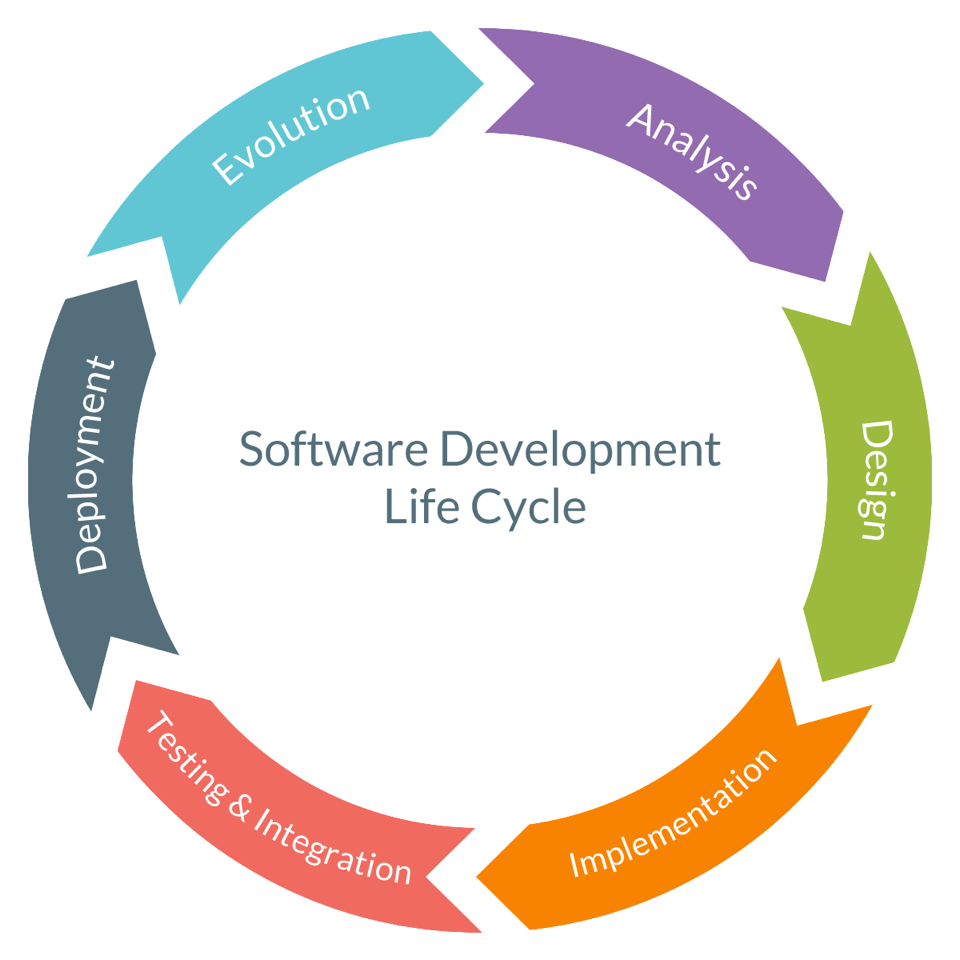
\includegraphics[width=0.2\textwidth]{figures/cycle.png}
    \end{figure}

    \textbf{S}ofware \textbf{D}evelopment \textbf{L}ife \textbf{C}ycle (\textbf{SDLC}) is the process followed for the development
    of a software product. Its goal: is to produce a software:
    \begin{itemize}
        \item with the \textbf{highest quality} (bug-free, stable, robust,
        extensible, following the customer's requirements, ...)
        \item for the \textbf{lowest cost} (money, time, man power, ...).
    \end{itemize}
\end{frame}


% What is git
\section{What is git?}
\begin{frame}{How people talk about git}
	\textbf{A lot} of the internet if about git related questions
	\begin{figure}
     	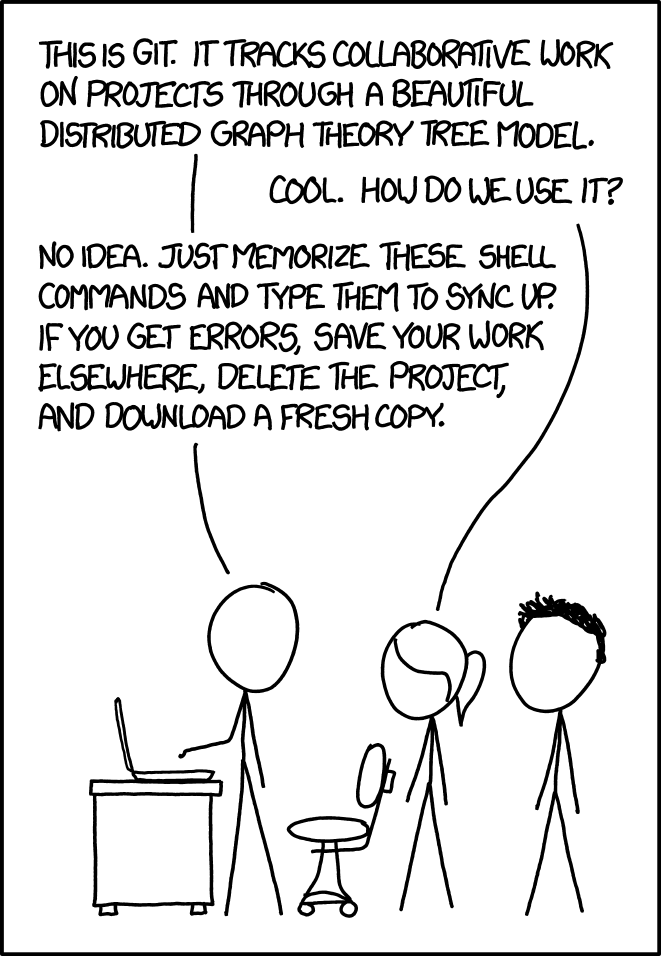
\includegraphics[width=0.3\textwidth]{figures/xkcd1.png}
     	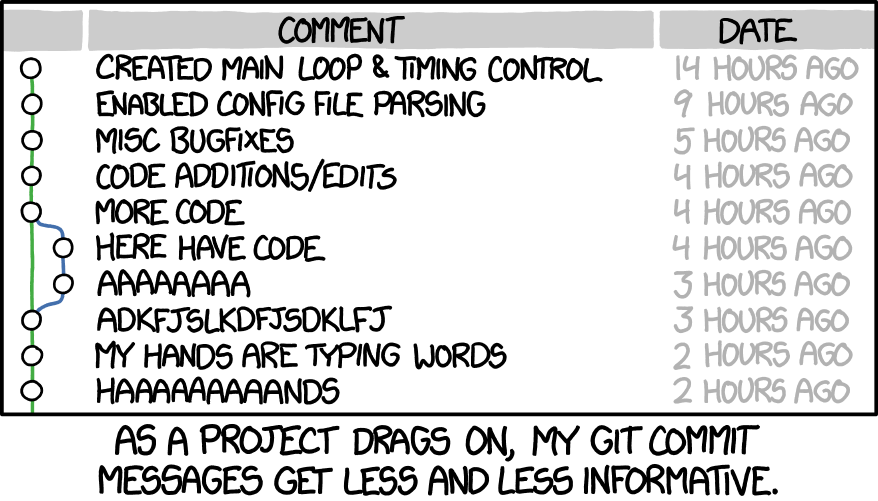
\includegraphics[width=0.3\textwidth]{figures/xkcd2.png}
     	
\includegraphics[width=0.3\textwidth]{figures/futurama.jpg}
     \end{figure}
\end{frame}


\begin{frame}{But what is it really?}
	git is a \textbf{V}ersion \textbf{C}ontrol \textbf{S}ystem (\textbf{VCS}).\\
	\textbf{VCS} are tools to manage and organize information changes in a code. They allow you to:
	\begin{itemize}
		\item work collaboratively
		\item work on several files
		\item work on several tasks
		\item keep track of your development
	\end{itemize}
	git is \textbf{distributed} (DVCS), $\neq$ SVN which is centralized:
	\begin{itemize}
		\item complete code base is stored on everyone's computer
		\item not dependent on network connection
		\item faster
		\item allows private work
	\end{itemize}
\end{frame}

\begin{frame}{Example}
	\begin{columns}
    	\column{.4\linewidth}
        Git is \textbf{big} and can be \textbf{complex} and \textbf{complicated}:\newline
        $\Longrightarrow$ \textbf{Use a proper client}
		\column{.6\linewidth}
		\begin{figure}
     		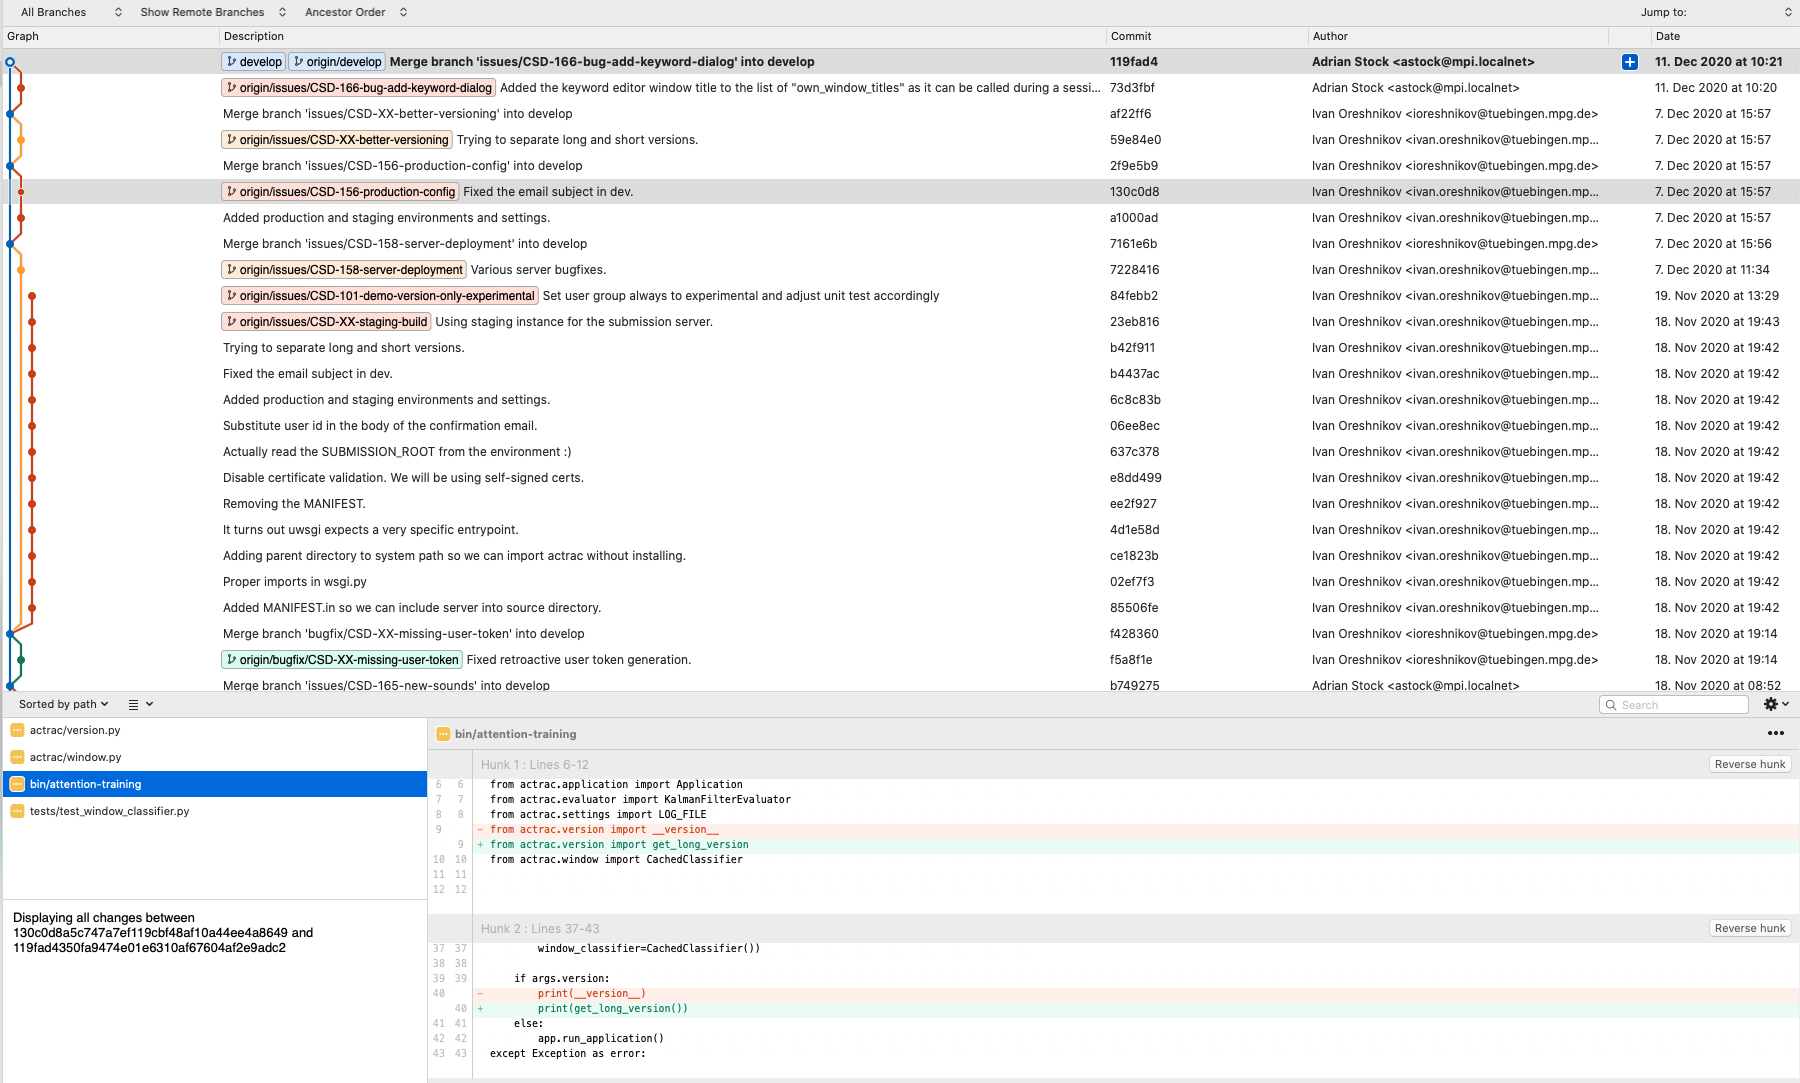
\includegraphics[width=\textwidth]{figures/git-general}
    		\end{figure}
	\end{columns}
\end{frame}


% Setting up git

\section{Setting up git}

\begin{frame}{Identity}

	\begin{tcolorbox}[colback=mpg-gray,colframe=mpg-green,title=Global settings]
	  {\tt \$ git config -{}-global user.name "John Doe"}\\
	  {\tt \$ git config -{}-global user.email "john.doe@tuebingen.mpg.de"}
	\end{tcolorbox}
	\begin{tcolorbox}[colback=mpg-gray,colframe=mpg-green,title=Note]
		\begin{itemize}
			\item Name/emails can be set for each individual repository.
			\item Name/emails can be fixed afterwards by history rewrite\\ ({\tt git filter-branch})
		\end{itemize}
	\end{tcolorbox}
\end{frame}

\begin{frame}{Ignore rules}
	Some files should not be part of the repository (temporary files, by-products, ...).

	Use a {\tt .gitignore} to ignore files \textbf{locally} or \textbf{globally}.
	\begin{tcolorbox}[colback=mpg-gray,colframe=mpg-green,title=Global .gitignore]
		{\tt \$ git config -{}-global core.excludesfile   \$HOME/.gitignore\_global}
	\end{tcolorbox}
	\begin{tcolorbox}[colback=mpg-gray,colframe=red!40!black,title=Warning]
		.gitignore is shared with other developers. Think carefully before making changes!
	\end{tcolorbox}
\end{frame}


\section{Tutorial}

\begin{frame}{Philosophy}
	\begin{columns}
    		\column{.6\linewidth}
		\begin{tcolorbox}[colback=mpg-gray,colframe=mpg-green,title=Branches]
			\begin{itemize}
				\item Branches are just pointers to commits
                \item Isolate implementation changes
				\item Switch contexts
			\end{itemize}
		\end{tcolorbox}
		\begin{tcolorbox}[colback=mpg-gray,colframe=mpg-green,title=Workflow]
			\begin{itemize}
				\item New dev. starts on feature branch
				\item Usually start on reference stable state
				\item Always merge from stable into less stable
				\item Develop almost always stable
				\item Master always stable
			\end{itemize}
		\end{tcolorbox}
		\column{.4\linewidth}
		\begin{figure}
     		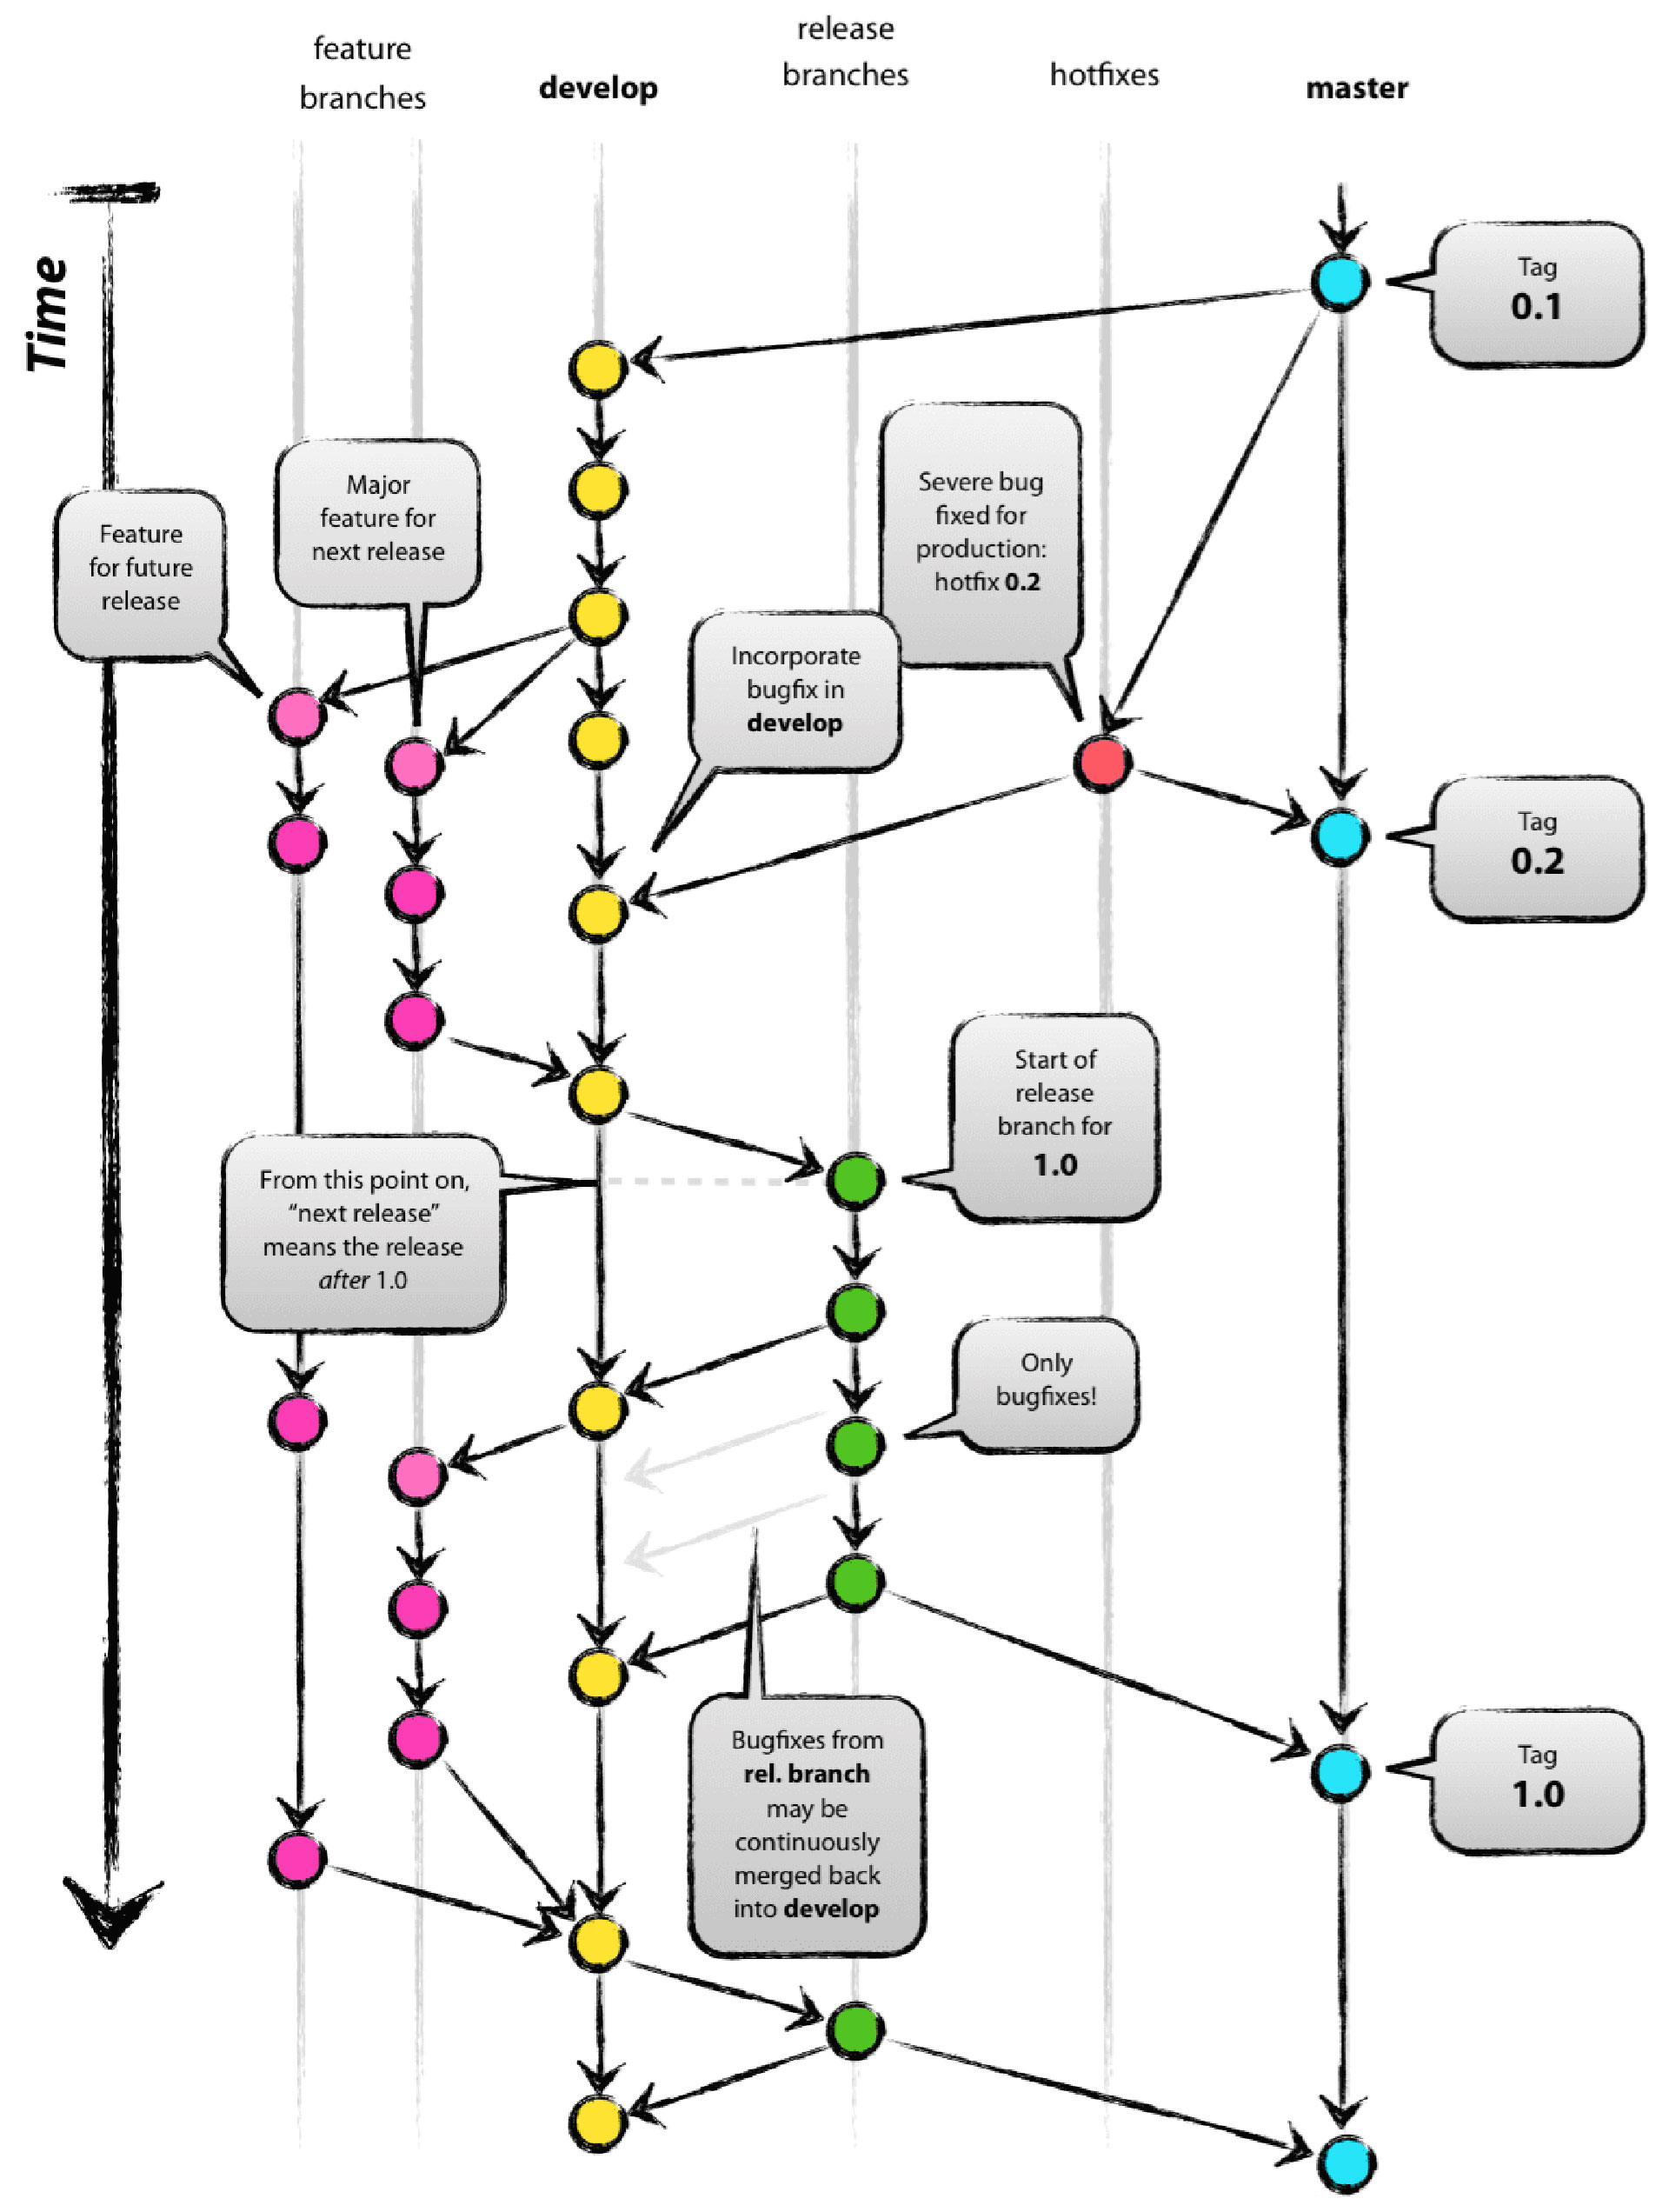
\includegraphics[width=0.8\textwidth]{figures/git-model.jpg}
    		\end{figure}
	\end{columns}
\end{frame}


\begin{frame}{Basic commands}
	\begin{itemize}
		\item Clone repository \hfill{\tt git clone url}
		\item Request changes from remote \hfill {\tt git fetch -{}-all}
		\item Work with branches \hfill {\tt git checkout my\_branch}
		\item Pull changes from the remote \hfill {\tt git pull}
		\item Show commit log \hfill  {\tt git log}
		\item Display the difference between commits \hfill {\tt git diff}
		\item See the status of the repository \hfill {\tt git status}
		\item Add files to the staging area \hfill {\tt git add -{}-update/-{}-all}
		\item Place non-committed changes to a shelf \hfill {\tt git stash apply/pop/drop}
		\item Merge last commit with the current one \hfill {\tt git commit -m ``Your message''}
		\item Push changes onto the remote \hfill {\tt git push}
	\end{itemize}
\end{frame}

\begin{frame}{Demo}
	\textbf{Task}: add your name to the README on a dedicated branch
		\begin{enumerate}
			\item Checkout the base branch on which you want to create you branch (double-click on the commit).The current branch appears in bold.
			\item Create a new branch by clicking on the {\tt Branch} button. You are now on this branch.
			\item Edit the files.
			\item {\tt Uncommited changes} appears in the history, click on it. Details appear in the lower part.
			\item Stage the changes you want to commit (checkbox or drag-and-drop).
			\item Click on the {\tt Commit} button, write your message, and commit.
			\item Push onto the remote.
    		\end{enumerate}
\end{frame}

\begin{frame}{Merging}
	Takes the union of changes (opposite action to branching).\\
	\begin{itemize}
		\item \textbf{Conflict resolution is part of life!}
		\item Only merge when the branch is \textbf{ready} (stable)
		\item Create new commit to keep topology (\textbf{no fast-forward})
		\item Delete branches after some time once they have been merged
	\end{itemize}

	\textbf{Task}: let's do some merging!
\end{frame}


\begin{frame}{Demo merging}
	\textbf{Task}: merge your branch onto develop and resolve conflicts if needed.
		\begin{enumerate}
			\item Checkout the base branch (develop) onto which you want to merge your feature branch.
			\item Click on the {\tt Merge} button.
			\item Select your feature branch and merge.
			\item If there are conflicts, the conflicted files will appear in the lower part with a warning sign.
			\item To resolve conflicts, righ-click on the file and choose {\tt Resolve Conflicts > Launch External Merge Tool}.
			\item A window with 3 panels should appear: content on the base branch (left), content on the feature  branch (right), and content that you want after the merge (bottom). This last panel can be edited directly.
			\item Save, close the merge tool, and stage the file that has been resolved.
			\item Do so for all the files containing conflicts, and commit.
			\item Push to the remote.
    		\end{enumerate}
\end{frame}

\begin{frame}{Rebasing}
	Moves the changes made on a branch onto another commit.
	\begin{figure}
     	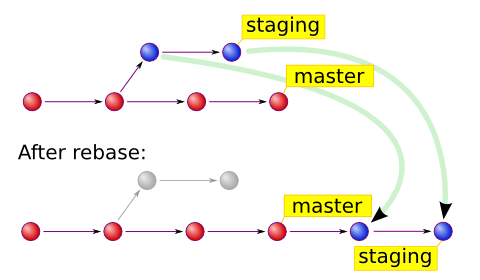
\includegraphics[width=0.5\textwidth]{figures/git-rebase.png}
    \end{figure}

    $\approx$ projects a branch implementation to the space \textbf{orthogonal} to other feature branches.
\end{frame}

\begin{frame}{Rebasing}
	Advantages:
	\begin{itemize}
		\item Keeps branch up-to-date with latest stable
		\item Keeps branch focused
		\item Make history shorter and therefore clearer
	\end{itemize}
	Workflow:
	\begin{itemize}
		\item Rebase your changes locally
		\item Make a diff between the local and remote branches: should be \textbf{orthogonal} to the feature implemented
		\item Force push to remote:

	\begin{tcolorbox}[colback=mpg-gray,colframe=mpg-green,title=Force push]
		{\tt \$ git push -f}
	\end{tcolorbox}
	\end{itemize}
\end{frame}

\begin{frame}{Dangers of rebasing}
	\begin{tcolorbox}[colback=mpg-gray,colframe=red!40!black,title=Warning]
		\begin{itemize}
			\item History is changed, so notify your colleagues working on this branch.
			\item All local copies should be synchronized:

					{\tt \$ git fetch -{}-all}\\
					{\tt \$ git checkout my\_branch}\\
					{\tt \$ git reset -{}-hard origin/my\_branch}
		\end{itemize}
	\end{tcolorbox}
	\textbf{Task}: let's do some rebasing!
\end{frame}

\begin{frame}{Demo rebasing}
	\textbf{Task}: rebase your branch on top of develop.
		\begin{enumerate}
			\item Checkout the feature branch you want to rebase.
			\item In the left panel, right-click on the base branch you want to rebase onto (develop) and select {\tt Rebase current changes onto ...}
			\item If there are conflicts, resolve them as you did when merging.
			\item At any point, you can stop the rebasing by selecting {\tt Actions > Abort Rebasing}.
			\item Once the conflicts have been resolved, select {\tt Actions > Continue Rebasing}.
			\item \textbf{Sanity check:} confirm that differences between the rebased local branch and the remote are \textbf{orthogonal} to the feature implemented.
			\item Force push to the remote.
    		\end{enumerate}
\end{frame}

\begin{frame}{Interactive Rebasing}
	Squashes the commits and rewrites history
	\begin{figure}
     	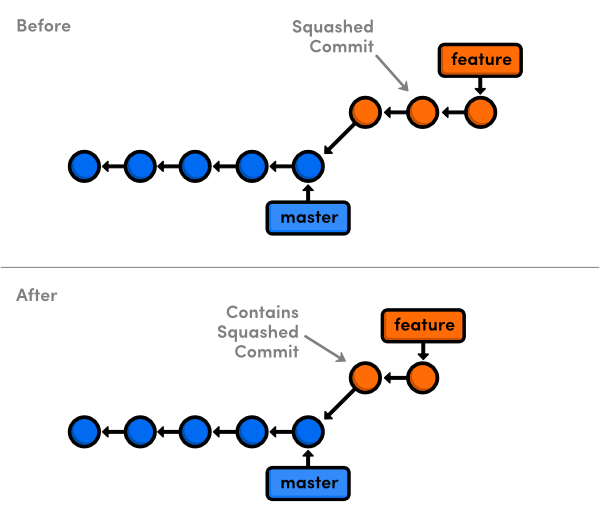
\includegraphics[width=0.5\textwidth]{figures/interactive-rebase.png}
    \end{figure}
	\begin{itemize}
		\item Takes the union of changes (opposite action to branching)
		\item Conflict resolution is part of the operation, so don't worry!
		\item Only merge when the branch is ready (green)
		\item Create new commit to keep topology (no fast-forward)
		\item Delete branches after some time once they have been merged
	\end{itemize}
\end{frame}

\begin{frame}{Advantages of interactive rebasing}
	\begin{itemize}
		\item Increases $S/N$ by diminishing history
		\item Makes branch scope easier to understand
		\item Makes branch easier to handle (rebase, merge, conflicts)
	\end{itemize}
	\textbf{Task}: let's do some interactive rebasing!
\end{frame}

\begin{frame}{Demo interactive rebasing}
	\textbf{Task}: squash the commits on your branch.
		\begin{enumerate}
			\item Checkout the feature branch you want to rebase.
			\item Select the branch root, i.e. parent commit of the first commit you want to squash.
			\item Right-click and select {\tt Rebase children of ... interactively}.
			\item Squash the commits, edit the commit messages, and confirm.
			\item \textbf{Sanity check:} confirm that there is \textbf{no difference} between the rebased local branch and the remote.
			\item Force push to the remote.
    		\end{enumerate}
\end{frame}

\begin{frame}{Cherry-picking}
	Apply changes introduces by some commit onto the current branch.
	\begin{figure}
     	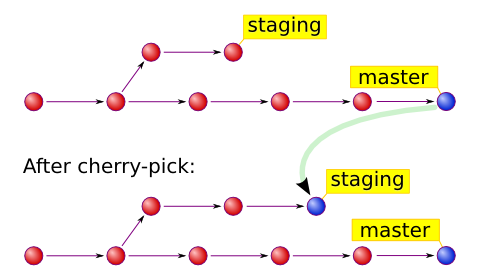
\includegraphics[width=0.5\textwidth]{figures/git-cherry-pick.png}
    \end{figure}
	\textbf{Task}: let's do some cherry-picking!
\end{frame}

\begin{frame}{Demo cherry-picking}
	\textbf{Task}: apply a change from another branch onto your branch.
		\begin{enumerate}
			\item Checkout your feature branch.
			\item Select the commit you want to cherry-pick.
			\item Right-click and select {\tt Cherry Pick}.
			\item If there are conflicts, resolve them as you did when merging.
			\item Push to the remote.
    		\end{enumerate}
\end{frame}


\begin{frame}{Last few tips}
	\begin{itemize}
		\item \textbf{Protect} master/develop against force push/developers!
		\item Empty folders are not tracked. Good practice is to use a {\tt .keep} file.
        \item By default, Sourcetree does not allow you to force push.
        The option must be first enabled in {\tt Settings > Advanced}.
		\item These concepts are sufficient for $\approx$ 90\% of what you will need to do.
	\end{itemize}
	\begin{figure}
     	
\includegraphics[width=0.3\textwidth]{figures/scary.png}
      \end{figure}
\end{frame}

\end{document}
